\chapter{Results and Discussions}\label{ch:results}
This chapter is organized as follows: Section \ref{sec:result_data} will discuss the main data used in this study, including an illustration of how to access it and the features it provides; Section \ref{sec:ch4_desc_stat} will discuss the results of the descriptive statistics; Section \ref{sec:ch4_morphological_analysis} will discuss the results on the morphological analyses; Section \ref{sec:ch4_structural_analysis} will discuss the results on the structural analyses; Section \ref{sec:ch4_topic_modeling_result} will discuss the results of the topic modeling; and Section \ref{sec:ch4_relating_islamic_texts} will discuss the results of relating the Qur'\=an to other Islamic texts and analyses. Finally, Section \ref{sec:ch4_limitations} will discuss the limitations of the models used in this study.
\section{Qur'\=an Data}\label{sec:result_data}
The main data used in this study is the digitized Qur'\=an data available through QuranTree.jl library by \citeA{asaad2021qurantree}. QuranTree.jl has both the Tanzil data\footnote{\url{https://tanzil.net/}} and the Qur'anic Arabic Corpus\footnote{\url{https://corpus.quran.com/}}, where the latter contains the morphological data of the Qur'\=an. These digital data will help in doing programmatic analyses of the Qur'\=an using Julia programming language. To see how to access this in QuranTree.jl in Julia, Figure \ref{fig:result_crps_tbl} shows the code for accessing the morphological data of the first \arb[trans]{'ayaT} \arb{'ayaT} of \arb[trans]{sUraTu 'l-fAti.haT} \arb{sUraTu 'l-fAti.haT}. Note that, the setup on how to install the said QuranTree.jl and other libraries and the Julia programming language is given in Appendix \ref{appendix:installation_libraries}.

Referring to Figure \ref{fig:result_crps_tbl}, the first line of the code, which has the code \texttt{using QuranTree}, loads the QuranTree library. The second line, which has the code \texttt{crps, tnzl = load(QuranData())}, loads both the morphological data and the Tanzil data of the Qur'\=an. The third line of the code converts these data into a tabular form. Finally, the fourth line of the code queries the first \arb[trans]{sUraT} \arb{sUraT} and the first \arb[trans]{'ayaT} \arb{'ayaT} of the morphological data of the Qur'\=an, the results of which are shown in succeeding lines with the heading indicating \texttt{Chapter 1} and \texttt{Verse 1}. Both the number 1 for Chapter 1 is indicated by \texttt{[1]} and \texttt{[1]}, respectively, in the code \verb|crps_tbl[1][1]| in Figure \ref{fig:result_crps_tbl}.

\begin{figure}[!t]
    \centering
    \includegraphics[width=\textwidth]{img/crps_tbl.png}
    \caption{\arb[trans]{sUraTu 'l-fAti.haT} \arb{sUraTu 'l-fAti.haT} morphological data}
    \label{fig:result_crps_tbl}
\end{figure}

The output of the code in Figure 1 as indicated by the lines starting with \texttt{\#} shows the morphological data of the \textit{basmallah} \arb[fullvoc]{bismi 'l-l_ahi 'l-ra.hm_ani 'l-ra.hImi}. In this data, there are five columns after the Row column. The \texttt{word} column indicates the word of the queried data, in this case the first \arb[trans]{'ayaT} \arb{'ayaT} of the first \arb[trans]{sUraT} \arb{sUraT}. According to this column, there are four words in the \textit{basmallah}. The second column, \texttt{part}, indicates the parts of the word. In this case, the first word, has two parts. These two parts is indicated by its \texttt{form} in the third column, which are \texttt{bi} a Roman encoding based on Buckwalter mapping which is decoded in Arabic as \arb{bi}, and the second part of the first word has the form in Roman encoding through Buckwalter as \texttt{somi} or decoded in Arabic as \arb[fullvoc]{smi}. The fourth column indicates the part-of-speech of the parts of the words. For the first word, \arb[fullvoc]{bismi}, its two parts are composed of Preposition \arb{bi} and a Noun \arb[fullvoc]{smi}, both of which are further described in the \texttt{features} column, which is the morphological features column. In this last column, it further tells the reader that the Preposition \arb{bi} is a prefix. In addition, the second part \arb[fullvoc]{smi} is the stem of the word \arb[fullvoc]{bismi}, with lemma indicated by \texttt{\{som} which is decoded as \arb{"ism}, and a root of \arb{smw}. There are still other features detailed in the morphological column for the second word \arb[fullvoc]{smi}, and this can be describe further using QuranTree.jl's \texttt{@desc} macro. The result of which is given in Figure \ref{fig:result_at_desc_basmallah}, which also show the other features such as the gender of the noun, in this case it is Masculine and is in Genitive case.

\begin{figure}[!t]
    \centering
    \includegraphics[width=\textwidth]{img/at_desc_basmallah.png}
    \caption{Morphological feature of the second part of the word \arb[fullvoc]{bismi}}
    \label{fig:result_at_desc_basmallah}
\end{figure}

The Quranic Arabic Corpus data which contain the morphological features discussed above, has the Qur'\=an texts represented as Buckwalter encoding, which is a character by character mapping of the Arabic orthographies of the Qur'\=an into a Roman letter. This encoding if decoded to Arabic matches exactly the Qur'\=an musaf. In fact, the Tanzil data which is also available in QuranTree.jl, exactly matches this data. The difference between the two is that the Tanzil data only contains the Arabic texts of the Qur'\=an broken down up until the \arb[trans]{'ayaT} \arb{'ayaT} only. Figure \ref{fig:result_tnzl_tbl} shows the Tanzil data queried through the QuranTree.jl for \arb[trans]{sUraTu 'l-fAti.haT} \arb{sUraTu 'l-fAti.haT}. The only difference between the two data in terms of presentation of the \arb[trans]{sUraT} \arb{sUraT} is that, the Quranic Arabic Corpus (in Figure \ref{fig:result_crps_tbl}) skips the \textit{basmallah} for all \arb[trans]{sUwar} \arb{sUwar} except for the first, \arb[trans]{sUraTu 'l-fAti.haT} \arb{sUraTu 'l-fAti.haT}, while the Tanzil data has it in every \arb[trans]{sUwar} \arb{sUwar}.

\begin{figure}[!t]
    \centering
    \includegraphics[width=\textwidth]{img/tnzl_tbl.png}
    \caption{\arb[trans]{sUraTu 'l-fAti.haT} \arb{sUraTu 'l-fAti.haT} Tanzil data}
    \label{fig:result_tnzl_tbl}
\end{figure}

The rich data available in QuranTree.jl opens up many possibilities for researchers to do programmatic analyses of the Qur'\=an. Especially on the use of Statistical modeling to understand its structure and patterns. This paper will demonstrate some of these possibilities. The data can be used to do morphological analyses, structural analyses, and even topic modeling. The data can also be used to do other analyses such as sentiment analysis, and other text analytics. 

\section{Descriptive Statistics}\label{sec:ch4_desc_stat}
The first statistical analysis is to describe the distribution of the data, through Descriptive Statistics. This statistical method is mainly used to summarize the data by looking at the central tendency, dispersion, and shape of the distribution of the data. The central tendency is a measure of the center of the data, which can be represented by the mean, median, and mode. The dispersion is a measure of how spread out the data is, which can be represented by the range, variance, and standard deviation.

The data in this case are the orthographies, parts of words, words, \arb[trans]{ayAt} \arb{ayAt}, and \textit{s\=urah} \arb{sUraT} of the Qur'\=an. The Qur'\=an is a collection of 114 \textit{s\=urah} \arb{sUraT} and 6,348 \arb[trans]{ayAt} \arb{ayAt}. Each \textit{s\=urah} \arb{sUraT} is made up of a number of \arb[trans]{ayAt} \arb{ayAt}, and each \arb[trans]{ayAt} \arb{ayAt} is made up of a number of words, which in turn is made of parts, and finally parts are made up of Arabic letters. These data as discussed in the previous section are available through the Quranic Arabic Corpus and the Tanzil data in the QuranTree.jl library.

As discussed in the Introduction of this thesis, the Qur'\=an has unique organizational structure unlike other scriptures. This has attracted both Muslims and non-Muslims to endeavor on understanding its structure. Most of the scholars have done this manually, going through each \arb[trans]{ayAt} \arb{ayAt} and \arb[trans]{sUraT} \arb{sUraT} of the Qur'\=an one at a time to find patterns that will at least convey why it is arranged as it is. However, this manual process is very tedious and time consuming, and hence other opportunities to understanding its structure has not yet been explored. Among those is undersanding the statistics of the counts of the words, \arb[trans]{AyAt} \arb{AyAt}, and \arb[trans]{suwar} \arb{suwar}. 

\begin{figure}[!t]
    \centering
    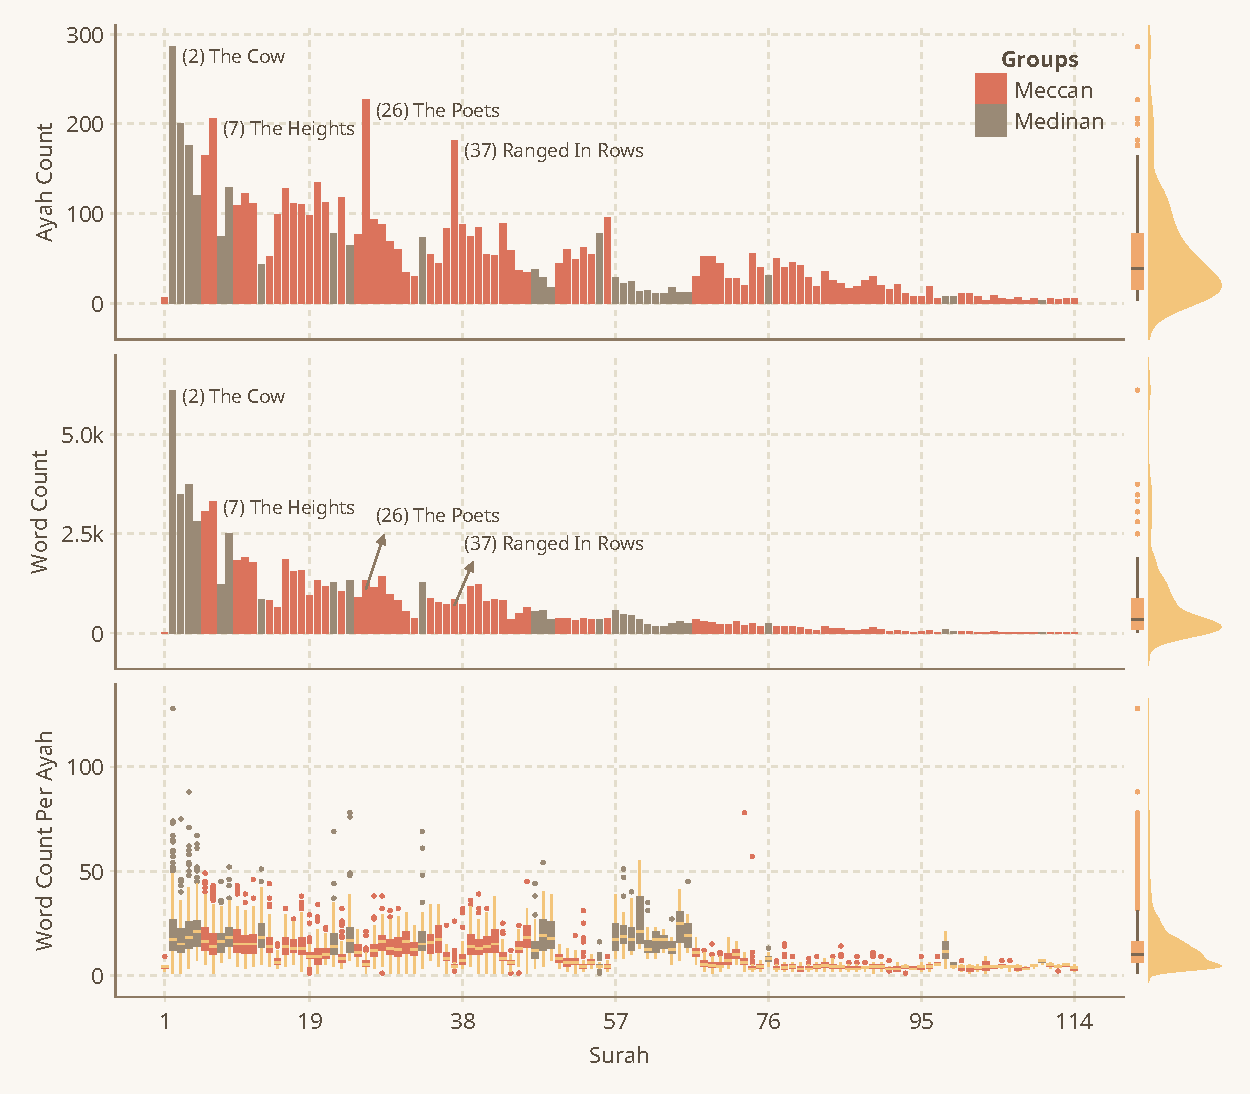
\includegraphics[width=\textwidth]{img/plot1.pdf}
    \caption{Distribution of Meccan and Medinan \arb[trans]{sUwar} \arb{sUwar}}
    \label{fig:result_ayah_word_count}
\end{figure}

Figure \ref{fig:result_ayah_word_count} shows the bar chart of the \arb[trans]{AyAt} \arb{AyAt} counts and word counts, and also the distribution of the word counts and character counts both per \arb[trans]{ayAt} \arb{ayAt}. In this figure, the geographical locations (Meccan or Medinan) of the \arb[trans]{sUraT} \arb{sUraT} based on the \arb[trans]{'asbAb 'alnuzUl} \arb{'asbAb 'alnuzUl} or the 'occasions/circumstances of revelation' are also indicated.

The first obvious pattern, which is known to Muslims, is the monotonically decreasing number of the \arb[trans]{ayAt} \arb{ayAt} after the first \arb[trans]{sUraT} \arb{sUraT}. This is true for both the bar charts of the \arb[trans]{ayAt} \arb{ayAt} count and the word count. An interesting pattern also is that, two \arb[trans]{suwar} \arb{suwar} has significant number of \arb[trans]{AyAt} \arb{AyAt} but with each \arb[trans]{ayAt} \arb{ayAt} having small number of words. These two \arb[trans]{suwar} \arb{suwar} are the \arb[trans]{sUraT} \arb{sUraT} 26th (\arb[trans]{sUraTu 'l-^su`arA'} \arb{sUraTu 'l-^su`arA'} or "the Poet") and 37th (\arb[trans]{sUraTu 'l-.sAffAt} \arb{sUraTu 'l-.sAffAt} or "the Ranged in Rows"), respectively. This can be confirmed even in the Medina Mushaf, where the first page for \arb[trans]{sUraTu 'l-^su`arA'} \arb{sUraTu 'l-^su`arA'} already contains 19 \arb[trans]{AyAt} \arb{AyAt}, and the \arb[trans]{sUraTu 'l-.sAffAt} \arb{sUraTu 'l-.sAffAt} contains 24 \arb[trans]{AyAt} \arb{AyAt} in its first page. This indicates that the said \arb[trans]{suwar} \arb{suwar} contain small number of words per \arb[trans]{ayAt} \arb{ayAt} shown in Figure \ref{fig:result_ayah_word_count}.

Moving on, the distribution of the words per \arb[trans]{ayAt} \arb{ayAt} and the characters per \arb[trans]{ayAt} \arb{ayAt} are shown in the third and fourth rows or plots of Figure \ref{fig:result_ayah_word_count}. It is indeed expected that these distributions are more or less identical, since it is expected that more words means more characters. The reason why the distribution of characters per \arb[trans]{ayAt} \arb{ayAt} is shown is to make it comparable to the work of \citeA{sinai2020oqs}, which will be compared later in Section. 

To interpret these distributions of word count per \arb[trans]{ayAt} \arb{ayAt} and the character count per \arb[trans]{ayAt} \arb{ayAt}, the x-axis is still the 114 \arb[trans]{suwar} \arb{suwar} of the Qur'\=an, while the y-axis is either the count of words (third row plot) per \arb[trans]{ayAt} \arb{ayAt} or the count of characters (fourth row plot) per \arb[trans]{ayAt} \arb{ayAt} in Figure \ref{fig:result_ayah_word_count}. Thus, each boxplot shown in these plots describes the distributions of the count of either the words or characters per \arb[trans]{ayAt} \arb{ayAt}. From these distributions, an interesting groups of distributions at around 57th \arb[trans]{sUraT} \arb{sUraT} to 66th \arb[trans]{sUraT} \arb{sUraT} are observed. These distributions while might be reasoned as easily seen because of its Medinan \arb[trans]{'asbAb 'alnuzUl} \arb{'asbAb 'alnuzUl} color, the mean of these are obviously higher than its surrounding \arb[trans]{sUraT} \arb{sUraT} as seen in the figure. In fact, these \arb[trans]{suwar} \arb{suwar} have lower number of \arb[trans]{ayAt} \arb{ayAt} compared to its surrounding \arb[trans]{suwar} \arb{suwar} (\textit{see} first plot and second plot of Figure \ref{fig:result_ayah_word_count}). Although, the number of words are more or less the same.

Further, it can be observed that the distributions of the Medinan \arb[trans]{suwar} \arb{suwar} tend to have higher mean as opposed to those in Meccan \arb[trans]{suwar} \arb{suwar}, which is indeed the case as seen in later discussions. In fact, as a prelude to this, if the order of the arb[trans]{suwar} \arb{suwar} is based on the \arb[trans]{'asbAb 'alnuzUl} \arb{'asbAb 'alnuzUl}, the observation that Medinan surah has higher number of word or character per \arb[trans]{ayAt} \arb{ayAt} can be seen in Figure \ref{fig:result_ayah_word_count_rev_order}. In this figure, the Medinan \arb[trans]{suwar} \arb{suwar} seen in the latter part of the \arb[trans]{'asbAb 'alnuzUl} \arb{'asbAb 'alnuzUl} clearly have higher mean counts and tend to have variable number of word or character counts per \arb[trans]{ayAt} \arb{ayAt}. This is again true especially when looking at the overall distributions of these categories across \arb[trans]{suwar} \arb{suwar} as in Figure \ref{fig:result_meccan_medinan_dist}.

\begin{figure}[!t]
    \centering
    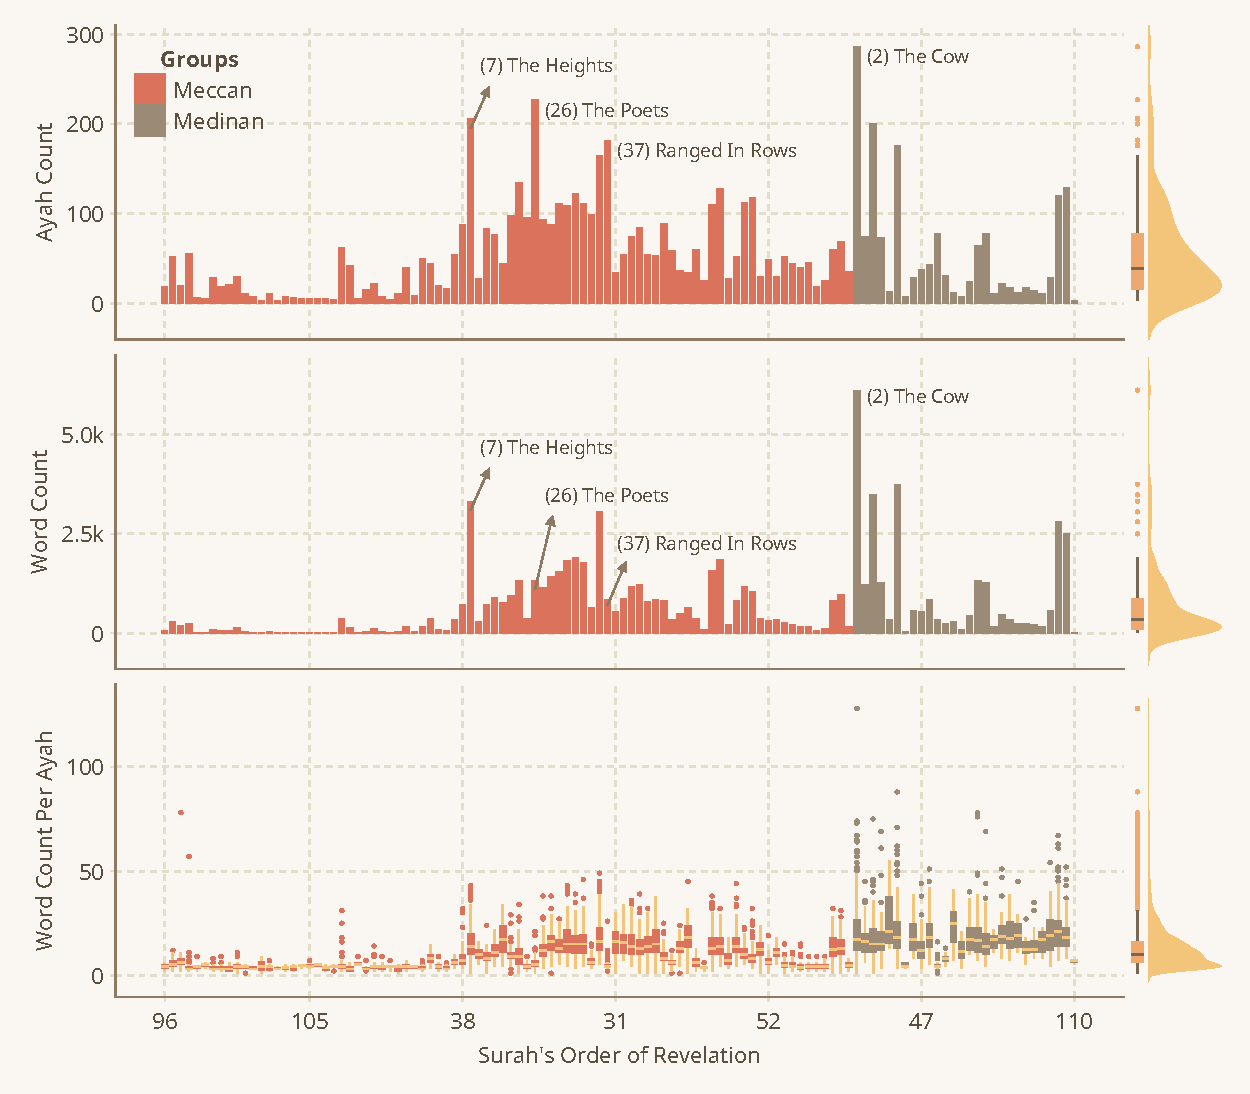
\includegraphics[width=\textwidth]{img/plot2.pdf}
    \caption{Statistics of the words and \arb[trans]{ayAt} \arb{ayAt} (verses) of the Qur'\=an according to revelation order}
    \label{fig:result_ayah_word_count_rev_order}
\end{figure}

\begin{figure}[!t]
    \centering
    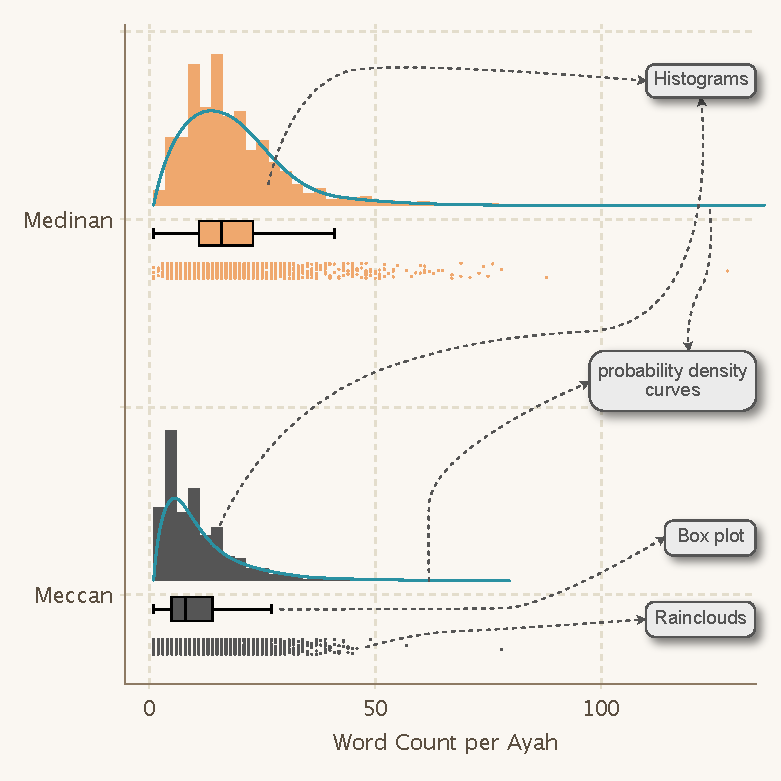
\includegraphics[width=\textwidth]{img/plot3.pdf}
    \caption{Distribution of Meccan and Medinan \arb[trans]{sUwar} \arb{sUwar}}
    \label{fig:result_meccan_medinan_dist}
\end{figure}

\begin{table}
    \caption{Descriptive statistics of the \arb[trans]{ayAt} \arb{ayAt} counts and the counts of its words}
    \label{tbl:desc_stats}
    \begin{tabularx}{\textwidth}[!h]{XXXX}
        \toprule
        Count Data&Mean&Median&Std. Deviation\\
        \midrule
        Ayahs&54.70&39&53.21\\
        Words&679.20&344&931.18\\
        Words per Ayah&10.27&8.23&6.35\\
        \bottomrule
    \end{tabularx}
\end{table}
\subsection{Comparison to Sinai's Inner-Chronology}
The work of \citeA{sinai2020oqs} investigated the same statistical distributions as in the previous section, but has focused from a non-traditionalist view by not basing on the \arb[trans]{'asbAb 'alnuzUl} \arb{'asbAb 'alnuzUl}, and instead mainly on the Qur'\=an's text itself using a transliteration data from Prof. Hans Zirker. The said data is not exactly the same as the one used in here, nor it is publicly verified as the one (Quranic Arabic Corpus and the Tanzil data) used in this study. Nonetheless, if indeed the said transliteration is exactly the same as the one used here once decoded to its Arabic form, the result should more or less be the same. However, while the preprocessing done by \citeA{sinai2020oqs} was not done in the analyses of the previous section, the result of the distributions should not deviate much. In the said study of \citeA{sinai2020oqs}, the findings suggest that there is inner-chronology of the Qur'\=an. This was concluded by the said author by looking at the mean verse length, which is more or less similar to the median verse length indicator used in boxplots of the third and fourth plots of Figures \ref{fig:result_ayah_word_count} and \ref{fig:result_ayah_word_count_rev_order}. Indeed, median is a better metric than mean in this case due to outlier counts seen in the boxplots in Figures \ref{fig:result_ayah_word_count} and \ref{fig:result_ayah_word_count_rev_order}. It is surprising though that he considered those with significant variance or coefficient variations (meaning those \arb[trans]{suwar} \arb{suwar} with very varied number of characters per \arb[trans]{ayAt} \arb{ayAt}) as possible later insertion to the Qur'\=an upon his closer inspection. It may sound polemic to disregard his findings or to attack it, but to be fair to Muslim traditionalists that to believe in such claim requires solid evidence from extant manuscripts and not just from someone's own interpretation of the statistics or literary styles of the \arb[trans]{ayAt} \arb{ayAt}. Indeed, the findings of Prof. Sina's can be categorized as \textit{theories} as it does not have supporting manuscripts that shows one. It may also be difficult to prove so as all Qur'\=anic extant manuscripts are consistent with the current one, including the controversial Sana'a Palimpest, where also Prof. Sinai was fair to admit in his own book \cite{sinai2017} that the said texts have. 

Furthermore, while it is healthy for the advancement of any studies including Qur'\=anic studies to have opposing views. For the case of \citeA{sinai2020oqs}, the premise of not considering \arb[trans]{'asbAb 'alnuzUl} \arb{'asbAb 'alnuzUl} shows a different structure as discussed in the preceding section.
\section{Morphological Analysis}\label{sec:ch4_morphological_analysis}
The second statistical analysis is to analyze the morphological features of the Qur'\=an. There are several ways to do this, and the easiest one is to find a particular word and study its morphologies. This will be the goal of this section, and the important word to study is the name of God in the Qur'\=an and that is \arb[trans]{'l-l_ah} \arb{'l-l_ah}. The root of this word is the \arb[trans]{Alh} \arb[novoc]{Alh}, and thus the morphologies of this root word will be studied and compared againts the \arb[trans]{'asbAb 'alnuzUl} \arb{'asbAb 'alnuzUl} or the 'occasions/circumstances of revelation.' Table \ref{tbl:result_Alh_morphologies} contains the complete list of morphologies of \arb[trans]{Alh} \arb[novoc]{Alh}. The first column in the said table lists the said morphologies, the second column lists its location in \arb[trans]{sUraT} \arb{sUraT} and \arb[trans]{'ayaT} \arb{'ayaT}, the third column lists the total number of \arb[trans]{'ayaT} \arb{'ayaT} that has the said morphology in the Qur'\=an, and the fourth column lists the percentage of \arb[trans]{'ayaT} \arb{'ayaT} whose \arb[trans]{'asbAb 'alnuzUl} \arb{'asbAb 'alnuzUl} is Mecca. The codes on how to generate this table in Julia using QuranTree.jl, Yunir.jl, and DataFrames.jl libraries are shown in Figure \ref{fig:result_Alh_morphologies}.

\begin{table}[!t]
    \begin{tabularx}{\textwidth}[!h]{cXcc}
        \toprule\\[-0.3cm]
        Morph. & Surah \& Ayah & Count & Meccan \% \\[0.2cm]
        \midrule\\[-0.4cm]
        \arb[fullvoc]{'l-l_ahi} & 1:1, 2:8, 2:23, $\cdots$, 104:6, 110:1, 110:2 & $710$ & 47\% \\[0.2cm]
        \arb[fullvoc]{llahi} & 1:2, 2:22, 2:98, $\cdots$, 71:13, 72:18, 82:19 & $122$ & 55\%\\[0.2cm]
        \arb[fullvoc]{'l-l_ahu} & 2:7, 2:10, 2:15, $\cdots$, 98:8, 112:1, 112:2 & $624$ & 39\% \\[0.2cm]
        \arb[fullvoc]{'l-l_aha} & 2:9, 2:26, 2:55, $\cdots$, 72:12, 96:14, 98:5 & $351$ & 30\% \\[0.2cm]
        \arb[fullvoc]{'il---a---_aha} & 2:133, 3:6, 6:106, $\cdots$, 45:23, 47:19, 73:9 & $17$ & 76\% \\[0.2cm]
        \arb[fullvoc]{'il---a---_ahu} & 2:163, 16:22, 18:110, $\cdots$ , 21:108, 29:46, 41:6 & $8$ & 88\% \\[0.2cm]
        \arb[fullvoc]{'il---a---_ahiN} & 3:62, 28:38, 38:65 & $3$ & 67\%\\[0.2cm]
        \arb[fullvoc]{|"'AlihaTaN} & 6:74, 18:15, 21:21, $\cdots$, 36:23, 37:86, 43:45 & $9$ & 100\% \\[0.2cm]
        \arb[fullvoc]{|"'Alihata} & 7:127, 21:36, 21:68, 71:23 & $4$ & 100\% \\[0.2cm]
        \arb[fullvoc]{'il---a---_ahaN} & 7:138, 18:14, 26:29 & $3$ & 100\%\\[0.2cm]
        \arb[fullvoc]{|"'Alihati} & 11:53, 11:54, 19:46, 25:42, 37:36, 37:91, 38:6, 46:22 & $8$ & 100\% \\[0.2cm]
        \arb[fullvoc]{|"'Alihatu} & 11:101 & $1$ & 100\% \\[0.2cm]
        \arb[fullvoc]{'il---a---_ahuN} & 14:52, 21:29, 43:84, 52:43 & $4$ & 100\% \\[0.2cm]
        \arb[fullvoc]{|"'AlihaTuN} & 17:42, 21:22, 21:43 & $3$ & 100\% \\[0.2cm]
        \arb[fullvoc]{'il---a---_ahi} & 20:97, 40:37, 114:3 & $3$ & 100\% \\[0.2cm]
        \arb[fullvoc]{--|"'Alihati}& 21:59, 21:62 & $2$ & 100\%\\[0.2cm]
        \arb[fullvoc]{|"'il---a---_ahuN} & 27:60, 27:61, 27:62, 27:63, 27:64 & $5$ & 100\% \\[0.2cm]
        \arb[fullvoc]{|"'AlihaTa} & 38:5 & $1$ & 100\% \\[0.2cm]
        \arb[fullvoc]{'alihatu} & 43:58 & $1$ & 100\% \\[0.2cm]
        \bottomrule
    \end{tabularx}
    \caption{Morphologies of \arb[novoc]{Alh} in the Qur'\=an}
    \label{tbl:result_Alh_morphologies}
\end{table}

The codes in Figure \ref{fig:result_Alh_morphologies} defines a Julia function called \verb|get_morphologies| from lines 5 to 25. The body of this function contains logics for extracting the morphologies of a given root word. At a high level, the logics has the following flow: it reads the morphological features of the root word \arb[novoc]{Alh}, then it lists down the chapter and verses containing this root word, and then compute the total number of \arb[trans]{AyAt} \arb{AyAt} that contain the given morphology of the given root word. Finally, it returns the output in tabular form that is presented in Table \ref{tbl:result_Alh_morphologies}. The defined \verb|get_morphologies| function can then be used to generate similar tables from other root words without rewriting those codes in lines 5 to 25 of Figure \ref{fig:result_Alh_morphologies}. Indeed, this is the beauty of programming, it can automate the manual process. For example, to generate similar table for the morphology of \arb{r.hm}, the code is as simple as shown in Figure \ref{fig:result_rHm_morphologies}, which shows only the first five morphologies of \arb{r.hm}.

\begin{figure}[!t]
    \centering
    \includegraphics[width=\textwidth]{img/morphologies_Alh.png}
    \caption{Julia code for generating Table \ref{tbl:result_Alh_morphologies}}
    \label{fig:result_Alh_morphologies}
\end{figure}

\begin{figure}[!t]
    \centering
    \includegraphics[width=\textwidth]{img/morphologies_rHm.png}
    \caption{Julia code for generating morphologies of \arb[novoc]{r.hm}}
    \label{fig:result_rHm_morphologies}
\end{figure}

From the result it can be observed that those these morphologies are purely under Meccan: \arb[trans]{'alihatu}  \arb[fullvoc]{'alihatu} - a masculine plural noun in nominative case (\textit{see} Figure \ref{fig:result_mfeat_43_58} for the codes on how to get these details in QuranTree.jl); \arb[trans]{|"'AlihaTa} \arb[fullvoc]{|"'AlihaTa} - a masculine plural noun in accusative case; \arb[trans]{|"'il---a---_ahuN} \arb[fullvoc]{|"'il---a---_ahuN} - a masculine singular noun in indefinite state and nominative case; \arb[trans]{--|"'Alihati} \arb[fullvoc]{--|"'Alihati} - a masculine plural noun in genitive case; \arb[trans]{'il---a---_ahi} \arb[fullvoc]{'il---a---_ahi} - a masculine singular noun in genitive case; \arb[trans]{|"'AlihaTuN} \arb[fullvoc]{|"'AlihaTuN} - a masculine plural noun in indefinite state and nominative case; \arb[trans]{'il---a---_ahuN} \arb[fullvoc]{'il---a---_ahuN} - similar to \arb[trans]{|"'il---a---_ahuN} \arb[fullvoc]{|"'il---a---_ahuN} with slightly different morphology; \arb[trans]{|"'Alihatu} \arb[fullvoc]{|"'Alihatu} - a masculine plural noun in nominative case; \arb[trans]{|"'Alihati} \arb[fullvoc]{|"'Alihati} - a masculine plural noun in genitive case; \arb[trans]{'il---a---_ahaN} \arb[fullvoc]{'il---a---_ahaN} - a masculine singular noun in indefinite state and accusative case; \arb[trans]{|"'Alihata} \arb[fullvoc]{|"'Alihata} - a masculine plural noun in accusative state, \arb[trans]{|"'AlihaTaN} \arb[fullvoc]{|"'AlihaTaN} - a masculine plural noun in indefinite state and accusative case.

\begin{figure}[!t]
    \centering
    \includegraphics[width=\textwidth]{img/mfeat_43_58.png}
    \caption{Julia code for describing morphological features of \arb[trans]{'alihatu} \arb{'alihatu}}
    \label{fig:result_mfeat_43_58}
\end{figure}

The last column in Table \ref{tbl:result_Alh_morphologies} contains the percentages of the Meccan \arb[trans]{AyAt} \arb{AyAt}, therefore among the \arb[trans]{AyAt} \arb{AyAt} that contain the morphologies of \arb[trans]{'l-l_ahi} \arb[fullvoc]{'l-l_ahi} is that 47\% of those are Meccan. This column was generated by the code in Figure \ref{fig:result_meccan_ratio}.

\begin{figure}[!t]
    \centering
    \includegraphics[width=\textwidth]{img/meccan_ratio.png}
    \caption{Julia code for generating last column of Table \ref{tbl:result_meccan_ratio}}
    \label{fig:result_meccan_ratio}
\end{figure}

Sample \arb[trans]{AyAt} \arb{AyAt} are given for Q43:59, Q21:59, and Q2:23. The first \arb[trans]{'ayaT} \arb{'ayaT} contains the only morphology for \arb[trans]{'alihatu} \arb[fullvoc]{'alihatu} in the Qur'\=an, which is highlighted in red. The context of this \arb[trans]{'ayaT} \arb{'ayaT} is that it the \textit{gods} (\arb[trans]{'alihatu} \arb[fullvoc]{'alihatu}) referred here are the dieties worshipped by the disbelievers. The one they cited here as \textit{him} is given in the previous  \arb[trans]{'ayaT} \arb{'ayaT} as Jesus \txarb{\fontspec{Scheherazade New} ﵇}, the son of Mary \txarb{\fontspec{Scheherazade New} ﵍}. 

\begin{bottomtitledframe}{Q43:58}
    \begin{center}
        \begin{arab}[fullvoc]
            min ((sUraTu 'l-zuxrufi)): waqAlUA |"'a\arbcolor[red]{'a_alihatu}nA xayruN 'am huwa mA .darabUhu laka 'illA jadalA bal hum qawmun xA.simUn
        \end{arab}
        \begin{arab}[trans]
            min ((sUraTu 'l-zuxrufi)): waqAlUA |"'a\arbcolor[red]{'a_alihatu}nA xayruN 'am huwa mA .darabUhu laka 'illA jadalA bal hum qawmun xA.simUn
        \end{arab}
    \end{center}
    From Surah \textit{Ornaments of Gold}: saying, 'Are our \textcolor{red}{gods} better or him?' --- they cite him only to challenge you: they are a contentious people ---
\end{bottomtitledframe}

The next Meccan \arb[trans]{'ayaT} \arb{'ayaT} is Q21:59, which contain the morphology for \arb[trans]{--|"'Alihati} \arb[fullvoc]{--|"'Alihati}, which refers to \textit{gods} or \textit{deities} of the disbelievers. In this \arb[trans]{'ayaT} \arb{'ayaT} the question is coming from disbelievers during the time of Abraham \txarb{\fontspec{Scheherazade New} ﵇}, after he destroyed the idols worshipped by his father and the disbelievers. Indeed, the not so common morphologies for \arb[novoc]{alh} refer to false gods and dieties and not to the true God that the Qur'\=an refers to. 

\begin{bottomtitledframe}{Q21:59}
    \begin{center}
        \begin{arab}[fullvoc]
            min ((sUraTu 'l-'anbiyA'i)): waqAlUA man fa`ala ha_a_dA bi\arbcolor[red]{--|"'Alihati}n'A 'innahu lamina 'l-.za_alimIna
        \end{arab}
        \begin{arab}[trans]
            min ((sUraTu 'l-'anbiyA'i)): waqAlUA man fa`ala ha_a_dA bi\arbcolor[red]{--|"'Alihati}n'A 'innahu lamina 'l-.za_alimIna
        \end{arab}
    \end{center}
    From Surah \textit{The Prophets}: They said, 'Who has done this to our \textcolor{red}{gods}? How wicket he must be!
\end{bottomtitledframe}

Finally, the example for the use of \arb[novoc]{alh} morphology to refer to the true God in the Qur'\=an is given in Q2:23, for \arb[trans]{'l-lahi} \arb[fullvoc]{'l-lahi}. Here the context is the challenge of Allah or God to the disbelievers to produce a single \textit{s\=urah} \arb{sUraT} or chapter like that in the Qur'\=an. This is indeed a challenge that is still valid until today, and no one has ever produced a single \textit{s\=urah} \arb{sUraT} like the Qur'\=an. If there was one, it should have been published in a reputable journal addressing this challenge. The problem with producing this is that it should be with the same eloquence and beauty of the Qur'\=an. This is indeed a challenge that is still valid until today, and no one has ever produced a single \textit{s\=urah} \arb{sUraT} like the Qur'\=an. This is part of the \arb[trans]{'al-'i`jAzu 'l-qur`an} \arb{'al-'i`jAzu 'l-qur`an} or \textit{the inimitability of the Qur'\=an}, which is one of the main reasons why the Qur'\=an is considered to be a miracle by the Muslims.

\begin{bottomtitledframe}{Q2:23}
    \begin{center}
        \begin{arab}[fullvoc]
            min ((sUraTu 'l-baqaraTi)): wa-'in kuntum fI raybiN mmimmA nazzalnA `alY_a `abdinA fa'tUA bisUraTiN mmin mmi_tlihi wa-"ad`UA ^suhada'A'akum mmin dUni \arbcolor[red]{'l-lahi} 'in kuntum .sa--_a--diqIna
        \end{arab}
        \begin{arab}[trans]
            min ((sUraTu 'l-baqaraTi)): wa-'in kuntum fI raybiN mmimmA nazzalnA `alY_a `abdinA fa'tUA bisUraTiN mmin mmi_tlihi wa-"ad`UA ^suhada'A'akum mmin dUni \arbcolor[red]{'l-lahi} 'in kuntum .sa--_a--diqIna
        \end{arab}
    \end{center}
    From Surah \textit{The Cow}: If you have doubts about the revelation We have sent down to Our servant, then produce a single surah like it --- enlist whatever supporters you have other than \textcolor{red}{God} --- if you truly [think you can].
\end{bottomtitledframe}

The results shown in Table \ref{tbl:result_Alh_morphologies} found several verses for the common morphologies of \arb[novoc]{alh}, while those rare ones have been found by the codes in Figure \ref{fig:result_Alh_morphologies}. In fact, the whole results in Table \ref{tbl:result_Alh_morphologies} were generated in under 5 seconds and few lines of codes from Figure \ref{fig:result_Alh_morphologies} and \ref{fig:result_meccan_ratio}. Had it been done manually, it would have taken days, weeks or even months. Plus the final results will likely have human errors, or at least it will need another person to verify the results, which too will take time. This is the main advantage of programming as it can automate such process with great accuracy, so long as the codes are accurate. Generating new morphologies for any given root can be done in just one line of code as in the first line of code in Figure \ref{fig:result_rHm_morphologies}.

% \begin{bottomtitledframe}{Q43:58}
%    Hello!
% \end{bottomtitledframe}



\section{Thematic Analysis}\label{sec:result_thematic_analysis}
From previous section, it was concluded that those morphologies that are unique to Meccan \arb[trans]{sUwar} \arb{sUwar} are considered to refer to false gods or deities worshipped by the disbelievers. Whereas those with common morphologies are considered to refer to the true God. Sample \arb[trans]{sUwar} \arb{sUwar} were given above for three \arb[trans]{ayaT} \arb{ayaT}, but it would be better to also understand the themes of \arb[trans]{AyAt} \arb{AyAt} for other morphologies, especially those that are common. However, doing this manually would be very tedious and time consuming, since the first morphology, \arb[trans]{'l-lahi} \arb[fullvoc]{'l-lahi}, contain 710 \arb[trans]{AyAt} \arb{AyAt}. Trying to summarize this manually would take so much time, and will also be prone to human error. How to automate then?

In Statistics and Machine Learning, there are techniques to do this mathematically. Among the basic method is what is called Latent Dirichlet Allocation (LDA), an algorithm that can produce keywords as topics from a given text. The algorithm is based on the idea that each document is a mixture of topics, and each topic is a mixture of words. The algorithm works by assigning each word in the document to a topic, and then updating the topic assignments based on the words assigned to each topic. This process is repeated until the topic assignments converge. The result is a set of topics, each represented by a set of words, that can be used to summarize the document. LDA has been effective for topic modeling and has been widely used in various applications, including text classification, information retrieval, and document clustering.

Another approach to topic modeling is using the BERT (Bidirectional Encoder Representations from Transformers) model, in layman's term, it is an artificial intelligence model that can understand the meaning of words in a sentence by looking at the context of the words around it. The idea is that BERT can generate a numerical representation of a word or a sentence, which can then be used to find similar words or sentences. Since it can be used to find similar words, it therefore can be used to find themes --- which groups similar words. This concept is called BERTopic. 

The third approach to topic modeling or thematic clustering is to use Generative Pre-trained Transformer (GPT) model. The idea is that GPT can generate a summary of a given text, and this summary can be used to find the themes of the text. This approach is similar to LDA, but it uses a different algorithm to generate the summary. The advantage of using GPT is that it can generate a more accurate summary than LDA, and it can also be used to generate summaries for longer texts. For many readers, ChatGPT is the most popular AI model. Indeed, this is the GPT model referred here. 

Among the three approaches mentioned, the third one is the best for the study as it can do everything the first two approaches do, but with human-readable summary and many GPT models have been trained on Qur'\=an data. There are many open-sourced GPT models that can be used, but those commercialized one are more accurate, such as the ChatGPT or the ClaudeAI. For this study, Claude 3.7 Sonnet GPT model is used.

\begin{listing2}[!t]
    \centering
    \includegraphics[width=\textwidth]{img/ayah_morph_extract.png}
    \caption{Julia code for generating last column of Table \ref{tbl:result_meccan_ratio}}
    \label{fig:result_thematic_analysis}
\end{listing2}

\begin{table}[!h]
    \begin{tabularx}{\textwidth}[!h]{cXcc}
        \toprule\\[-0.3cm]
        Morph. & Surah \& Ayah & Count & Meccan \% \\[0.2cm]
        \midrule\\[-0.4cm]
        \arb[fullvoc]{'l-l_ahi} & Divine Unity \& Singularity (Tawhid) [6:164, 28:88, 2:163]; Faith \& Belief (Iman) [49:15, 65:11]; Divine Guidance \& Revelation [2:2, 5:48]; Prophet \& Messengers [2:136, 48:29]; The Day of Judgement \& Afterlife [2:281, 68:34]; Moral \& Ethical Teachings [16:90, 5:1]; Stories of Previous Nations [47:10]; Relationship Between Allah \& Creation [50:16, 51:56]; Rules \& Legislation [62:9, 4:2]; Struggle \& Perseverance [22:78, 2:155] & $710$ & 47\% \\[0.2cm]
        \arb[fullvoc]{llahi} & Divine Sovereignty \& Ownership [2:284, 3:109, 3:129]; Divine Attributes [4:170, 31:26, 4:139, 9:91]; Creator \& Sustainer [6:1, 35:1]; Purpose of Worship [53:62, 22:31]; Divine Judgement \& Authority [22:56, 24:64, 3:129]; Gratitude \& Praise [1:2, 6:1, 34:1, 35:1]; Divine Will \& Power [14:4, 3:129]; Submission to Allah [2:112, 4:125] & $122$ & 55\%\\[0.2cm]
        \arb[fullvoc]{'l-l_ahu} & Divine Unity \& Singularity (Tawhid) [112:1, 2:255, 2:116, 10:68]; Divine Sovereignty \& Power [7:54, 10:3]; Divine Knowledge [3:29, 9:94]; Divine Justice [40:20, 3:57]; Divine Guidance [2:213, 24:46, 57:25]; Divine Will \& Decree [14:27, 5:48]; Divine Names \& Attributes [59:24, 24:35]; Relationship with Believers [98:8]; Divine Creation \& Sustenance [23:14, 7:54]  & $624$ & 39\% \\[0.2cm]
        \arb[fullvoc]{'l-l_aha} & Divine Unity \& Singularity (Tawhid) [7:59, 19:36, 98:5]; Divine Attributes [49:16, 9:5, 2:284]; Obedience to Allah \& His Messenger [4:59, 64:12, 48:17]; Piety \& God Conciousness [3:102, 2:194, 8:25]; Reward \& Punishment [47:12, 40:17, 22:14]; Prayer, Charity, \& Righteous Deeds [98:5]; Stories of Prophets \& Past Nations [11:50, 11:61]; Faith \& Belief [49:10]; Justice \& Fairness [16:90] & $351$ & 30\% \\[0.2cm]
        \arb[fullvoc]{'il---a---_aha} & 2:133, 3:6, 6:106, $\cdots$, 45:23, 47:19, 73:9 & $17$ & 76\% \\[0.2cm]
        \arb[fullvoc]{'il---a---_ahu} & 2:163, 16:22, 18:110, $\cdots$ , 21:108, 29:46, 41:6 & $8$ & 88\% \\[0.2cm]
        \arb[fullvoc]{'il---a---_ahiN} & 3:62, 28:38, 38:65 & $3$ & 67\%\\[0.2cm]
        \arb[fullvoc]{|"'AlihaTaN} & 6:74, 18:15, 21:21, $\cdots$, 36:23, 37:86, 43:45 & $9$ & 100\% \\[0.2cm]
        \arb[fullvoc]{|"'Alihata} & 7:127, 21:36, 21:68, 71:23 & $4$ & 100\% \\[0.2cm]
        \arb[fullvoc]{'il---a---_ahaN} & 7:138, 18:14, 26:29 & $3$ & 100\%\\[0.2cm]
        \arb[fullvoc]{|"'Alihati} & 11:53, 11:54, 19:46, 25:42, 37:36, 37:91, 38:6, 46:22 & $8$ & 100\% \\[0.2cm]
        \arb[fullvoc]{|"'Alihatu} & 11:101 & $1$ & 100\% \\[0.2cm]
        \arb[fullvoc]{'il---a---_ahuN} & 14:52, 21:29, 43:84, 52:43 & $4$ & 100\% \\[0.2cm]
        \arb[fullvoc]{|"'AlihaTuN} & 17:42, 21:22, 21:43 & $3$ & 100\% \\[0.2cm]
        \arb[fullvoc]{'il---a---_ahi} & 20:97, 40:37, 114:3 & $3$ & 100\% \\[0.2cm]
        \arb[fullvoc]{--|"'Alihati}& 21:59, 21:62 & $2$ & 100\%\\[0.2cm]
        \arb[fullvoc]{|"'il---a---_ahuN} & 27:60, 27:61, 27:62, 27:63, 27:64 & $5$ & 100\% \\[0.2cm]
        \arb[fullvoc]{|"'AlihaTa} & 38:5 & $1$ & 100\% \\[0.2cm]
        \arb[fullvoc]{'alihatu} & 43:58 & $1$ & 100\% \\[0.2cm]
        \bottomrule
    \end{tabularx}
    \caption{Morphologies of \arb[novoc]{Alh} in the Qur'\=an}
    \label{tbl:result_Alh_morphologies_theme}
\end{table}

\section{Rhythmic Analysis}\label{sec:result_rhythmic_analysis}
\section{Theory of Concentric Structure}
One of the specific items for the second objective of this paper is on the theory of concentrism, and how can this be formulated statistically, and what are the insights that can be extracted. The idea of the theory of concentrism is that a given texts with define partition follows a ring or concentric structure, which is a literary form where the text is organized in such a way that it mirrors itself around a central point. This means that the beginning and ending sections correspond to each other, moving inward until the center of the text, which often contains the main message or theme. This particular pattern was observed by linguistic experts that it got documented in a book by \citeA{farrin2014structure}. This theory can be defined mathematically as follows:

\begin{defn}[\it Concentric]\label{defn:concentric}
    Let $\mathscr{D}$ be a collection of texts, then $\mathscr{D}$ is said to have a \textit{concentric} or \textit{ring} structure if and only if $\exists\;\mathscr{A}_i\subseteq\mathscr{D},\mathscr{C}\subseteq\mathscr{D},$ and $\mathscr{A}_i^{*}\subseteq\mathscr{D},i\in\mathbb{N}_1$; and that these sets are arranged as follows in $\mathscr{D}$:  $\mathscr{A}_1,\cdots,\mathscr{A}_n,\mathscr{C},\mathscr{A}_1^{*},\cdots,\mathscr{A}_n^{*}$, such that $\mathscr{A}_i^{*}$ \underline{mirrors} $\mathscr{A}_i$ in semantic, and that $\mathscr{C}$ is the center texts of the document $\mathscr{D}$ that is \underline{not related} to both $\mathscr{A}_i$ and $\mathscr{A}_i^{*}$.
\end{defn}

The underlined words above will be used in the next section, because mathematically it begs further definition on what we mean by "mirrors" and "not related" mathematically. This will be defined in the next section. Now, another pattern that was observed by \citeA{farrin2014structure} as chiasmus, which is basically \textit{ring} structure but the second half of the ring after the center is the "complement" or "reversal" of the first half of the document before the center. The following is its mathematical definition.

\begin{defn}[\it Chiasmus]\label{defn:chiasmus}
    Let $\mathscr{D}$ be a collection of texts, then $\mathscr{D}$ is said to have a \textit{concentric} or \textit{ring} structure if and only if $\exists\;\mathscr{A}_i\subseteq\mathscr{D},\mathscr{C}\subseteq\mathscr{D},$ and $\mathscr{A}_i^{*}\subseteq\mathscr{D},i\in\mathbb{N}_{geq 1}$; and that these sets are arranged as follows in $\mathscr{D}$:  $\mathscr{A}_1,\cdots,\mathscr{A}_n,\mathscr{C},\mathscr{A}_1^{c},\cdots,\mathscr{A}_n^{c}$, such that $\mathscr{A}_i^{c}$ is the \underline{complement} or \underline{reversal} of $\mathscr{A}_i$ in semantic, and that $\mathscr{C}$ is the center texts of the document $\mathscr{D}$ that is \underline{not related} to both $\mathscr{A}_i$ and $\mathscr{A}_i^{c}$.
\end{defn}
There are other structures that can be observed in the Qur'\=an, like \textit{parallelism} where themes are repeated in other \arb[trans]{sUraT} \arb{sUraT}; and \textit{segment structure}, where a particular segment starts and ends with similar phrases or themes, creating a bracket around the content; but, these other structures are not studied in this paper. Apart from this, there is also the "mathematical patterns" of the Qur'\=an which has been extensively studied by \citeA{rashad1981}, but this is also not studied in this paper.
\subsection{Bayesian Optimization}\label{sec:bayes-opt}
From Defn. \ref{defn:concentric} and \ref{defn:chiasmus}, it both states that, a document $\mathscr{D}$ may only be considered \textit{concentric} or \textit{chiasmus} if and only if "there exist", denoted by the symbol $\exists$. Indeed, subset of texts $\mathscr{A}_i$s, $\mathscr{C}$, and $\mathscr{A}_i^{*}$ or $\mathscr{A}_i^{\text{c}}$ are all determined manually by the investigator. In this study, we propose to automate the determination of these subsets of texts of document $\mathscr{D}$, and this is through the use of an optimization algorithm called Bayesian Optimization. The idea behind Bayesian optimization is that it approximates the objective function with a \textit{surrogate} function, and using this surrogate to find the global maximum or minimum of the objective function. Furthermore, it does this by fitting the surrogate function to the objective function in as few input points or iteration as possible. As such, an \textit{acquisition} function is needed for choosing smartly the next input points to be used for fitting the surrogate. Using these components, a Bayes' Theorem is used in fitting the surrogate.

To do this, a \textit{global objective function} must be defined, for this study, the cosine similarity discussed in the previous section will be used as the said cost function that will either be maximized or minimized. The core model for this optimization is the Gaussian Process defined below.
\subsubsection{Surrogate Function}
The surrogate function aims to approximate the objective function. In Bayesian, optimization, the surrogate function is defined by the Gaussian process (GP).
\begin{defn}[\it Gaussian Process]\label{defn:gp}
    Let $Y_1,Y_2,\cdots,Y_T$ be sequence of random variables such that $Y_t\in\mathbf{Y}$, then the sequence is a \textit{Gaussian process} (GP) if and only if $\mathbf{Y}\overset{\mathrm{iid}}{\sim}\mathcal{N}(\boldsymbol{\mu}, \boldsymbol{\Sigma})$.
\end{defn}
\begin{defn}[\it Parameter Space]\label{defn:parameter_space}
    Let $\mathbf{s}_i\in\mathscr{D}$ be a word embedding of an \arb[trans]{'ayaT} \arb{'ayaT} in document $\mathscr{D}$, which can be a \arb[trans]{sUraT} \arb{sUraT}, group of \arb[trans]{suwar} \arb{suwar}, or group of \arb[trans]{'Ayat} \arb{'Ayat} within a \arb[trans]{sUraT} \arb{sUraT}. Further, suppose $\mathscr{A}_i,\mathscr{C},\mathscr{A}_i^{*}\subseteq\mathscr{D}$ such that $\mathscr{A}_i:=\{\mathbf{s}_{i,1},\cdots,\mathbf{s}_{i,n}\},\linebreak\mathscr{C}:=\{\mathbf{s}_{n+1},\cdots,\mathbf{s}_{n+c}\}$, and $\mathscr{A}_i^{*}:=\{\mathbf{s}_{i,(n+c+1)},\cdots,\mathbf{s}_{i,(n+c+n)}\}$, then the \textit{parameters} to be optimized are assigned to $\mathbf{v}:=[n,c]^{\text{T}}$, and since $n,c,m\in\mathbb{N}_{\geq 2}$, then the \textit{parameter space} is $\mathscr{P}:=\mathbb{N}_{\geq 2}\times\mathbb{N}_{\geq 2}\times\mathbb{N}_{\geq 2}=(\mathbb{N}_{\geq 2})^3$, so that $\mathbf{v}\in\mathscr{P}$. 
\end{defn}
\begin{defn}[\it Semi-Circle Cost Function]\label{defn:semi_circle_cost}
    From Defn. \ref{defn:parameter_space}, let $r_1$ to denote that $\mathscr{A}_i$ is "related" to $\mathscr{A}_i^{*}$, and $r_2$ to denote that $\mathscr{A}_i$ is "reversal" of $\mathscr{A}_i^{*}$, such that $\eta:=\{r_1,r_2\}$, then  the \textit{semi-circle} cost function between $\mathscr{A}_i$ and $\mathscr{A}_i^{*}$ is defined as:
    \begin{equation}
        \operatorname{\gamma}_{a}(\mathbf{v};\mathscr{A}_i,\mathscr{A}_i^{*},\eta):=\begin{cases}
            \frac{1}{n}\sum_{k=1}^{n}\cos\left(\theta_{\mathbf{s}_{i,k};\mathbf{s}_{i,n+l}}\right),&\text{if}\;\eta=r_1\\
            1-\frac{1}{n}\sum_{k=1}^{n}\cos\left(\theta_{\mathbf{s}_{i,k};\mathbf{s}_{i,n+l}}\right),&\text{if}\;\eta=r_2\\
        \end{cases}
    \end{equation}
\end{defn}
\begin{defn}[\it Center Cost Function]\label{defn:center_cost}
    From Defn. \ref{defn:parameter_space}, the \textit{center} cost function is defined as:
    \begin{equation}
        \operatorname{\gamma}_{b}(\mathbf{v};\mathscr{A}_i,\mathscr{C},\mathscr{A}_i^{*}):=2-\frac{1}{nc}\sum_{k=1}^{n}\sum_{l=1}^{c}\cos\left(\theta_{\mathbf{s}_{i,k};\mathbf{s}_{n+l}}\right)-\frac{1}{nc}\sum_{k=1}^{n}\sum_{l=1}^{c}\cos\left(\theta_{\mathbf{s}_{n+l};\mathbf{s}_{i,n+c+k}^{*}}\right).
    \end{equation}
\end{defn}
\begin{defn}[\it Global Cost Function]\label{defn:global_cost}
    From Defn. \ref{defn:parameter_space}-\ref{defn:center_cost}, the \textit{global} cost function is defined as:
    \begin{equation}
        \operatorname{\gamma}_{g}(\mathbf{v};\mathscr{A}_i,\mathscr{C},\mathscr{A}_i^{*},\eta):=\operatorname{\gamma}_{a}(\mathbf{v};\mathscr{A}_i,\mathscr{A}_i^{*},\eta)+\operatorname{\gamma}_{b}(\mathbf{v};\mathscr{A}_i,\mathscr{C},\mathscr{A}_i^{*})
    \end{equation}
\end{defn}
\begin{defn}[\it Optimal Parameters] From Defn. \ref{defn:global_cost}, the optimal parameters would be:
\begin{equation}
    \hat{\mathbf{v}}:=\underset{n,c}{\arg\min}\operatorname{\gamma}_{g}(\mathbf{v};\mathscr{A}_i,\mathscr{C},\mathscr{A}_i^{*},\eta),
\end{equation}    
\end{defn}
\begin{prop}\label{prop:hypedist}
    Let $\mathscr{P}$ be the parameter space and suppose $\gamma(\mathbf{v})\overset{\mathrm{iid}}{\sim}\mathcal{N}(m(\mathbf{v}),k(\mathbf{v},\mathbf{v})), \linebreak\forall \mathbf{v}\in\mathscr{P}$, then for any $\boldsymbol{\delta}:=[\gamma(\mathbf{v}_1),\cdots,\gamma(\mathbf{v}_n)]^{\top}$, $\boldsymbol{\delta}\overset{\mathrm{iid}}{\sim}\mathcal{N}_n(\mathbf{m},\mathbf{K})$, where 
    \begin{equation}
        \mathbf{m}:=[m(\mathbf{v}_1),\cdots,m(\mathbf{v}_n)]^{\top}
    \end{equation}
    and
    \begin{equation}
        \mathbf{K}:=\left[\begin{matrix}
        k(\mathbf{v}_1,\mathbf{v}_1)&\cdots&k(\mathbf{v}_1,\mathbf{v}_n)\\
        \vdots&\ddots&\vdots\\
        k(\mathbf{v}_n,\mathbf{v}_1)&\cdots&k(\mathbf{v}_n,\mathbf{v}_n)\\
        \end{matrix}\right]
    \end{equation}
\end{prop}
\begin{proof}
    The proof follows from the proof of Theorem 1.2.9 of \citeA{muirhead2005}.
\end{proof}
\begin{remark}
    From Proposition \ref{prop:hypedist} and Definition \ref{defn:gp}, $\boldsymbol{\delta}$ is a GP.
\end{remark}
\begin{prop}\label{prop:jointpdf}
    From Proposition \ref{prop:hypedist}, suppose $\boldsymbol{\delta}_{*}:=[\gamma(\mathbf{v}_{n+1}),\cdots,\gamma(\mathbf{v}_{n+p})]^{\top}$, such that $\boldsymbol{\delta}_{*}\overset{\mathrm{iid}}{\sim}\mathcal{N}_p(\mathbf{m}_*,\mathbf{K}_*)$ then 
    \begin{equation}
        \left[
        \begin{matrix}
            \boldsymbol{\delta}\\
            \boldsymbol{\delta}_{*}\\
        \end{matrix}
        \right]\overset{\mathrm{iid}}{\sim}
        \mathcal{N}_{n+p}\left(\left[
        \begin{matrix}
            \mathbf{m}\\
            \mathbf{m}_{*}\\
        \end{matrix}
        \right],\left[
        \begin{matrix}
            \mathbf{K}&\mathbf{K}_{*}\\
            \mathbf{K}_{*}^{\top}&\mathbf{K}_{**}\\
        \end{matrix}
        \right]\right)
    \end{equation}
\end{prop}
\begin{proof}
    Let $\mathbf{u}:=[\boldsymbol{\delta},\boldsymbol{\delta}_{*}]^{\top}$, then $\mathbf{u}=[\gamma(\mathbf{v}_1),\cdots,\gamma(\mathbf{v}_{n+p})]^{\top}$. Further, since $\mathbf{\gamma}(\mathbf{v}_i)\overset{\mathrm{iid}}{\sim}\mathcal{N}(m(\mathbf{v}_i),k(\mathbf{v}_i,\mathbf{v}_i)),\forall i\in\mathbb{N}_{\leq n+p}$, then the joint distribution of the $\gamma(\mathbf{v}_i)$s, i.e. $\mathrm{Pr}(\mathbf{u})$, follows from the proof of Theorem 1.2.9 of \citeA{muirhead2005}.
\end{proof}
\begin{cor}\label{cor:condpdf}
From Proposition \ref{prop:jointpdf}, let $\mathbf{m}$ and $\mathbf{m}_{*}$ be zero vectors, then the following conditional distribution is true:
    \begin{equation}\label{eq:gp_updater}    \boldsymbol{\delta}_*\mid\boldsymbol{\delta}\overset{\mathrm{iid}}{\sim}\mathcal{N}_{p}(\mathbf{K}_{*}^{\top}\mathbf{K}^{-1}\boldsymbol{\delta},\mathbf{K}_{**}-\mathbf{K}_{*}^{\top}\mathbf{K}^{-1}\mathbf{K}_{*}).
\end{equation}
\end{cor}
\begin{proof}
    The proof follows by reversing the condition from $\mathbf{X}_1\mid\mathbf{X}_2$ to $\mathbf{X}_2\mid\mathbf{X}_1$ of the proof of Theorem 1.2.11 of \cite{muirhead2005}.
\end{proof}
\begin{defn}[\it Lower Confidence Bound]\label{defn:lcb}
    Let $m(\mathbf{v})$ be the mean of the GP, then the Lower Confidence Bound (LCB) notated as $\xi$ is given by
    \begin{equation}
        \xi(\mathbf{v}\mid\zeta):=m(\mathbf{v})-\zeta k(\mathbf{v},\mathbf{v}),
    \end{equation}
    where $\zeta$ is the balancing factor.
\end{defn}
The \textit{global cost} computed from the global cost function in Defn. \ref{defn:global_cost} is approximated by the Gaussian process (the surrogate function) defined in Defn. \ref{defn:gp} through Proposition \ref{prop:hypedist}. So that, for any new observed global cost computed from the new parameter input $\mathbf{v}$, chosen by the acquisition function defined in Defn. \ref{defn:lcb}, the joint distribution with the previous global cost is given in Proposition \ref{prop:jointpdf}. Therefore, computing for the conditional distribution of the new global costs conditioned on previous global cost is given in Corollary \ref{cor:condpdf}. The process of acquiring new parameter candidate and computing the global cost is done iteratively. The algorithm converges until there is no significant changes on the new parameter candidate relative to the preceding parameter candidate, or alternatively, until a specified maximum iteration.
\begin{center}
    \textcolor{red}{add theoretical Bayes theorem computations here}
\end{center}
\subsection{Discussions on Islamic Philosophy of Qur'\=an's Structural Analysis}
\newpage
\section{Topic Modeling}\label{sec:ch4_topic_modeling_result}
\subsection{Latent Dirichlet Allocation}
\subsection{Bidirectional Encoder Representation from Transformer}
\subsection{Generative Pre-Trained Transformer}
\section{Relating to other Islamic Texts and Analyses}\label{sec:ch4_relating_islamic_texts}
\subsection{Retrieval-Augmented Generation Approach}
\section{Limitations of the Models}

\section{Advantages of Computation}
